\section{ACE-M3: Quantitative microscopy}\label{ace-m3-quantitative-microscopy}
Thus far, ACE-M2 has been a resounding success. Every one of the samples which
we have launched appears to work as we expected: dyes are bright, colloidal
suspensions show variations in intensity. But most importantly, we are able to
watch quite clearly the early stages of phase separation, as described in
previous posts. So far, so good; we have a great \emph{qualitative}
understanding of what is happening so far.

Upcoming experiments will look at the phase-separating samples in greater
detail, with hope to quantify the rate of phase separation---something we have
been able to do at larger lengthscales with the BCAT series of experiments,
using photography and some image processing. But what we have never been able to
figure out reliably is the concentration of particles in the two phases after
phase separation. Unfortunately, the photos we take with the camera flash are
not \emph{linear} in relating intensity the image to particle concentration.
Why? Imagine photographing clouds; you can't really tell how thick the cloud
layer is just by its brightness; if a lower cloud passes in front of another
one, even if the total cloud thickness doubles, the light (usually) doesn't fall
by exactly half.

These concentrations after the samples phase separate are important for us to
understand some fundamental physics, test existing theories in a new regime, and
be able to place our samples in the context of other systems. And they cannot be
measured on the ground, where sedimentation may take place---which will
inherently change the measured concentrations. So being able to quantify the
relationship between brightness in the microscope and particle density is
extremely important for the science we want to explore, and something we were
never quite able to do with the BCAT experiments.

ACE, however, uses fluorescence, a process that is linear. If you collect light
from a sample well like we have on orbit, if the particle density is twice, the
total brightness should also be twice. You might recall that we already launched
a series of particle suspensions, which was intended to serve this purpose. We
are looking at that data now, and hopefully that should work. But doing careful
experiments means that we are always happy to run independent controls,
cross-checks, and different systems to verify what we think we are seeing. A
different method to quantify the brightness vs. concentration relationship would
therefore be very useful.

Fortunately, we have been given a great opportunity to send up more samples with
the next round of ACE-M experiments, ACE-M3 which (at the moment) is set to
launch in the fall aboard SpaceX-4. Preparing for this experiment involved a
number of unique challenges:
\begin{enumerate}
\item We were only given the go-ahead a couple of weeks ago, after a bit of begging and pleading to squeeze us on board the next rocket! Fortunately, NASA and the great folks at ZIN agreed to make a little more space. So we had five new samples we could prepare---and only a few days to prepare them.
\item Because of the last-minute nature of the sample prep, we were restricted to the materials that were already approved as safe with a new set of sample cells (slightly different in construction from the ones we use on ACE-M2, but no time to update the loading procedures). But luckily, those materials include dyes that are the same colors as the particles, namely those based on fluorescein and rhodamine.
\item We need the samples we prepare to reflect similar optical behavior as the particles, suspensions and mixtures we already launched with ACE-M2. If they are too different, say involving different filters and lenses, then the results might not apply directly to the system whose physical behavior we want to quantify better on orbit.
\end{enumerate}

\subsection{Sample preparation and
characterization}\label{sample-preparation-and-characterization} 
I chose the rhodamine dyes, for the reason that it is red / pink, and our
particles are pink, so I figured it was a decent place to start. Two samples
with the same fluorescence should be the same color in different lighting
conditions. I then took some rhodamine dye and dispersed in water, and ended up
with a very dark red color, like a red wine, and I could barely see through it.
So it seems like it had way too much dye, and I started diluting it out by
factors of 10. But if we want to control the dye concentration, how can you
assess that? Unfortunately, weighing the dye out is not very accurate. I started
with a few mL of water, but the amount of dye is only a couple of milligrams,
and our balance only reads to 0.1 mg, so the error on the dye concentration is
inherently no better than a few percent.

Moreover, how do we predict what the brightness will be in a fluorescence
microscope? Obviously, we could use a fluorescence microscope, but if that is
the instrument we are testing, we would prefer an independent way to measure the
brightness. The best way would be to use a fluorometer, a specialized instrument
that sends in a beam of light at a user-selectable wavelength (i.e. color), and
then measures the amount of fluorescence emitted. Unfortunately, we don't have
such an instrument, and the ones in the chemistry department are not that
convenient.

\subsubsection{UV-Vis absorption
spectroscopy}\label{uv-vis-absorption-spectroscopy} We do, however, have a UV-Vis absorption spectrometer. This instrument sends
light into the sample one color at a time, scanning over a large range of
wavelengths, and records the amount of light passing through. These instruments
are very carefully calibrated, and ours has a second reference light beam, so
the data it outputs is a very careful, quantitative measure of absorbance. Why
does this help? Because in order for light to be re-emitted as fluorescence, it
must be absorbed at a lower wavelength. And by conservation of energy, doubling
the fluorescence emission will lead to double absorption; it's also a linear
relationship (barring some specific quantum mechanical effects which I don't
expect to be sensitive to). So assessing the peak of the absorption gives us a
way to characterize concentration.
\begin{figure}[h]
\begin{center}
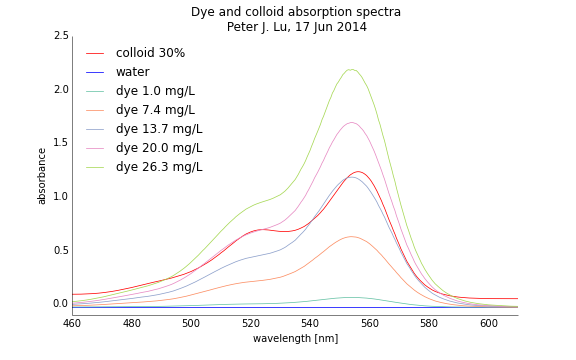
\includegraphics[width=\columnwidth]{./images/2014_06_17_dye/dye_colloid_abs_140617.png}
\end{center}
\caption{UV-Vis spectra}
\end{figure}

First, I ran a sample of just plain distilled water. There should be no peaks in
the absorption spectrum, and it should be basically be flat through the entire
range of wavelengths (460 to 610 nm), as it is colorless---and therefore has no
fluorescence---and transparent. Indeed, this is what I see, shown by the blue
curve in the absorption spectra. I then ran the colloidal sample at 30\% volume
fraction, right in the middle of the range we have on orbit; its spectra has a
nice peak at about 555 nm---which is why the samples appear pink: they absorb
green light, and the absence of green light (e.g. on a color wheel) is pink /
magenta.

Then I ran concentrations of the rhodamine dye; fortunately, the main peak in
the absorption spectrum is very, very close to that of the particles, shown with
the curves in the other colors. You can see how close the peaks are for the
colloids (red) and the dye at a concentration of 13.7 mg/L. This is very, very
fortunate, because it shows how the optical behavior of the dye is an excellent
proxy for the spectral characteristics of our particles!

So by a bit of trial an error, I found the rough dye concentration corresponding
to the brightness of our 30\% colloid sample. Then with some careful sample
prep, I spaced them out linearly over the range of brightness that spans what I
expect the colloids on orbit will (other colored lines in the plot), so we will
learn about the camera and imaging system with parameters similar to what we
will use for the colloids.

\subsubsection{Samples to be launched}\label{samples-to-be-launched}

Here's the final list of samples we submitted to ZIN / NASA:

\begin{center}
\begin{tabular}{c|c}
\textbf{Sample} & \textbf{Dye concentration}\\
\hline
plu\_M3A & 1.05 mg/L\\
plu\_M3B & 7.36 mg/L\\
plu\_M3C & 13.7 mg/L\\
plu\_M3D & 20.0 mg/L\\
plu\_M3E & 26.3 mg/L\\
\end{tabular}
\end{center}

\subsection{Testing linearity}\label{testing-linearity}
\begin{figure}
\begin{center}
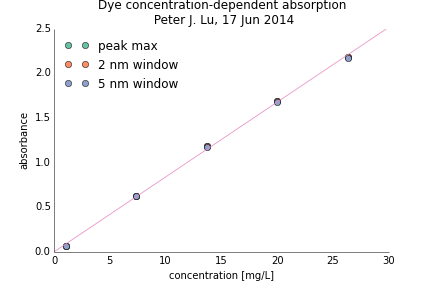
\includegraphics[width=\columnwidth]{./images/2014_06_17_dye/dye_concs_abs_140617.png}
\end{center}
\caption{Absorption vs. concentration}
\end{figure}
To check the linearity of the fluorescence intensity, I measured the height
(absorbance) of each peak at 554 nm, and plotted it as a function of
concentration (from the sample preparation). There are several ways to measure
the peak: reading off the top value, or averaging over a few nm around the
maximum. In all cases, the points fall on top of each other, as seen in the
figure at right, where the different ways of measuring peak height are
indistinguishable. And, critically, the points all fall along a straight line
(purple in the figure), which extrapolates to very close to the origin. These
data show very carefully that the relationship between absorbance---and
therefore fluorescence---is linear with dye concentration, which have similar
spectral characteristics to the colloidal particles we have launched.


This is exactly as we would hope for a good set of standard samples, to use to
then explore and calibrate the imaging system properly, using a different
chemistry while still in the same physical realm (in terms of fluorescence
intensity) that we are interested in for our colloidal samples. So we are very
excited to launch these as a part of the ACE-M3 experiment!

Finally, here is the code from the second plot, with the linear fit to the
{raw data}:
\begin{lstlisting}[showspaces=false,showtabs=false,language=python,basicstyle=\ttfamily\footnotesize,columns=fixed,frame=tlbr,float]
from pylab import *
import csv
import prettyplotlib as ppl

dye_concs_data = []
for row1 in csv.reader(open('peak_summary_130615.txt'), delimiter='\t'): 
    dye_concs_data.append(row1)
header1 = dye_concs_data[0]
water_blank = dye_concs_data[1]
values1 = array(dye_concs_data[2:]).astype(np.float)
concs=values1[:,0]
window5nm = values1[:,2]
linfit = polyfit(concs, window5nm, 1)
fitrange =[0,30]

figure(figsize=(6,4))
for i in range (1,4):
    ppl.plot(concs,values1[:,i],'o')
ppl.plot(fitrange,polyval(linfit,fitrange),'-')
xlabel('concentration [mg/L]')
ylabel('absorbance')
title('Dye concentration-dependent absorption\n Peter J. Lu, 17 Jun 2014')
xlim([0,30])
ylim([0,2.5])
lg= legend(['peak max','2 nm window','5 nm window'],'upper left')
lg.draw_frame(False)
savefig('dye_concs_abs_140617.pdf')
\end{lstlisting}   %  class="language-python"

